% \vspace{-12mm}
% \raggedbottom
\section{Evaluation} \label{sec:eval}

In this section we present a thorough evaluation of our task-inference attacks on MTL models trained for differing use cases across both vision and language domains. We showcase our attacks' success and study their performance when the adversary has access to training samples (i.e. \textbf{strong}) and when they only have access to fresh samples from the challenge task (i.e. \textbf{weak}). Additionally, we attempt to understand the factors that lead to task-inference leakage by observing how task-inference changes as a function of the MTL model's generalization loss. Additional experiments and figures can be found in Appendix~\ref{appdx:eval}. The results we present are underscored by our attacks' efficiency, taking as few as four samples per task and requiring \emph{only black-box query access} to the shared representation. In our experiments, this translates to each black-box query and task-inference prediction taking roughly \emph{one tenth of a second} on a single RTX 4090 GPU.

% \vspace{-2mm}
\subsection{MTL Training} 
In this study, we consider the original instantiation of MTL training which is described in the seminal work on the topic of MTL~\cite{caruana-1997-multitask}. We highlight that this MTL algorithm is a slight variation of centralized FedSGD~\cite{mcmahan2017FLoriginal}, one of the baseline algorithms in the original paper on collaborative learning. For all of our models, we allow all tasks to share all but the task-specific classification heads. In our experiments, the shared representation takes the form of a neural network, and the classification heads are linear. During MTL training, we perform a forward pass and route each embedding vector to its corresponding task-specific layer. Thus, in the backward pass, the loss from \textit{all} tasks is used to train the shared encoder, while only the loss from each particular task is used to train each linear layer. Algorithm~\ref{alg:mtl_training} shows the general training loop we use for MTL. In practice, we use AdamW~\cite{loshchilov-2017-adamw} for our \texttt{Update} step, and we perform shuffling over tasks and batching for efficiency. Additionally, when there is sufficient data available per task, we randomly subsample data from each task for each training epoch. 

\begin{algorithm}[h]
    \caption{Multitask Learning Training Loop}
    \label{alg:mtl_training}
    \begin{algorithmic}[1]
       \State {\bfseries Input:} A shared representation $h_\theta$, $T$ task-specific layers $\{g_{\beta_1}, \dots, g_{\beta_T}\}$, a training set split by task $D~=~\{(X_{1}, y_1 ) \dots (X_{T}, y_T )\}$, number of training rounds $t$, a loss function $\mathcal{L}$
       \For{$i \in [t]$}
            \State $\ell_{\textit{MTL}}$ $\gets 0$ \Comment{Initialize multitask loss}
            \For{$j \in [T]$} 
                \State $p_j \gets g_{\beta_j} ( \: h_{\theta}(\: X_j \:) \:)$ \Comment{Get predictions for task $j$}
                \State $\ell_{\textit{MTL}} \gets \ell_{\textit{MTL}} + \frac{1}{T} \mathcal{L}(p_{j}, y_j)$
            \EndFor
            \For{$j \in [T]$} \Comment{Update each task specific layer}
                \State $\beta_j \gets \texttt{Update} \left( \beta_j, \: \nabla_{\beta_j} \ell \right)$ 
            \EndFor
            \State $\theta \gets \texttt{Update} \left(\theta, \:  \nabla_{\theta} \ell \right)$ \Comment{Update shared representation}
        \EndFor
        \Return $h_\theta$
    \end{algorithmic}
\end{algorithm}

Since the number of samples per task can be smaller than the embedding dimension, we use several regularization techniques (detailed in Appendix~\ref{appdx:training}) to keep the task-specific linear layers from overfitting to noisy embeddings early during MTL training. To summarize, we use large values for weight decay, or $L_{2}$ regularization, learn a bottleneck on the shared representation to decrease the embedding dimension, normalize gradients~\cite{chen-2018-gradnormalization} across tasks during model updates, apply clipping to gradients, and, in our vision experiments, apply standard augmentations to training images.



                
            
                
            


% \begin{algorithm}[H]
%     \caption{MTL Training Loop}
%     \label{alg:simple_fedsgd_mtl}
%     \begin{algorithmic}[1]
%         \State {\bfseries Input:} Learning rates $\eta_{1}, \eta_{2}$, number of iterations , batch of tasks $\{D_i\}_{i=1}^M$
%         \State {\bfseries Initialize:} Shared representation parameters $\theta$ for $h$, task-specific linear layers $\{g_i\}_{i=1}^M$ with parameters $\{\beta_i\}_{i=1}^M$
%         \For{$t = 1, 2, \ldots, T$}
%             \State $\nabla \theta \gets 0$ \Comment{Initialize gradient for shared representation}
%             \For{task $i = 1, 2, \ldots, M$}
%                 \State Sample batch $(x_i, y_i) \sim D_i$ \Comment{Sample data from task $i$}
%                 \State $h \gets h_{\theta}(x_i)$ \Comment{Compute shared representation}
%                 \State $\hat{y}_i \gets g_i(h; \beta_i)$ \Comment{Task-specific prediction}
%                 \State $\mathcal{L}_i \gets \ell(y_i, \hat{y}_i)$ \Comment{Task-specific loss}
%                 \State $\nabla \theta_i \gets \nabla_{\theta} \mathcal{L}_i$ \Comment{Compute gradient for shared representation}
%                 \State $\nabla \beta_i \gets \nabla_{\beta_i} \mathcal{L}_i$ \Comment{Compute gradient for task-specific layer}
%                 \State $\nabla \theta \gets \nabla \theta + \nabla \theta_i$ \Comment{Aggregate gradients for shared representation}
%                 \State $\beta_i \gets \beta_i - \eta \nabla \beta_i$ \Comment{Update task-specific parameters}
%             \EndFor
%             \State $\theta \gets \theta - \eta \nabla \theta$ \Comment{Update shared representation with aggregated gradient}
%         \EndFor
%         \State \Return $\theta$, $\{\beta_i\}_{i=1}^M$ \Comment{Return final model parameters}
%     \end{algorithmic}
% \end{algorithm}

\subsection{Models and Datasets}


\subsubsection{Vision Models} In our vision experiments, we use ResNet models~\cite{ResNet} of differing sizes as the shared representation for MTL. The ResNet architecture has gained widespread adoption across computer vision applications due to its computational efficiency and high performance on a variety of datasets. This model architecture makes use of residual connections, which stabilize training and convergence to help maintain high utility when trained on large image datasets. When available, such as in our CelebA experiments, we use larger ResNet models which are pretrained on the ImageNet~\cite{imagenet} dataset from the PyTorch~\cite{paszke2019pytorch} library.


\subsubsection{Language Models} For our language experiments, we use the BERT~\cite{devlin2018bert}  architecture as the shared representation. In particular, we use the downsized variants of BERT~\cite{bertsmall_1, bertsmall_2} which are pretrained on MNLI~\cite{MNLI} for downstream sequence classification.

% on the StackOverflow~\cite{stackoverflow} topic classification dataset.


\subsubsection{Vision Datasets} We evaluate our task-inference attacks on both the CelebA~\cite{liu-2015-celeba} faces dataset and the Federated EMNIST (FEMNIST)~\cite{caldas-2019-leafbenchmark} handwritten character and images dataset. CelebA contains high-resolution images of celebrities, each with a unique identifier, and 40 facial attributes with binary labels. The FEMNIST dataset contains 28x28 grayscale images of 62 different types of handwritten characters. In our experiments on CelebA, we split the dataset into tasks by person and by facial attribute for each of the two MTL use cases we consider. We split FEMNIST by writer and train an MTL model for character recognition, personalized to each writer's hand-drawn images.

% strong = {'quantile': [0.5, 0.75, 0.9],
%  'tpr': [0.5947079128689237, 0.32012346055772567, 0.13629684764814576],
%  'fpr': [0.40533447265625, 0.179931640625, 0.06378173828125],
%  'acc': [0.5946867201063368, 0.5700959099663628, 0.5362575546834478]}

% weak = {'quantile': [0.5, 0.75, 0.9],
%  'tpr': [0.532562255859375, 0.27862548828125, 0.11383056640625],
%  'fpr': [0.46746826171875, 0.22142036109449761, 0.08619359928409948],
%  'acc': [0.5325469970703125, 0.5286025635933762, 0.5138184835610753]}
%TPR at 0.010009765625 FPR (Strong):  0.027587890625

\subsubsection{Language Datasets} To evaluate our attack in the language setting, we use the Stack Overflow~\cite{stackoverflow} dataset, which consists of posts from the Stack Overflow website with corresponding ratings, user ID, and topic tags for each post. In our evaluation, we split the posts into tasks by user ID and by topic for each of the MTL use cases. 
% \subsubsection{Synthetic Data}

% \

% Vision: CelebA facial attribute, FEMNIST character classification for personalizationm, CelebA for multiple objectives
% Language: Stack Overflow posts for topic classification, both personalization and multiple learning obejctives
% Synthetic: Describe how we generate the labelings or refer to section and discuss there



% \vspace{-1mm}
\subsection{Metrics}

To measure the performance of our task-inference attacks, we use metrics that are commonly found in the inference attack literature~\cite{carlini-2022-lira, zarifzadeh2024lowcostmia, ye-2022-enhanced_mi, kandpal2023userinference}. In particular, we analyze the ROC curves of our attack, which measure the relationship between true positive rate (TPR) and false positive rate (FPR). As summary statistics, we report the area under the ROC curve, or AUC, as well as the TPR at fixed low FPR (e.g. 1\%). Our evaluation distinguishes between two adversarial settings: a \textbf{strong} adversary with access to training samples and a \textbf{weak} adversary limited to auxiliary data from the challenge task that was never seen during training. Thus, we present ROC curves for each adversary. Additionally, we highlight that our attacks can be performed in a purely black-box setting. This results in the adversary not necessarily having sufficient knowledge to select the threshold that yields an optimal tradeoff between TPR and FPR. So, we also report the (TPR, FPR) pairs when thresholding our test statistics at the 50th, 75th, and 90th percentiles.


% \begin{figure}[h]
%     \centering
%     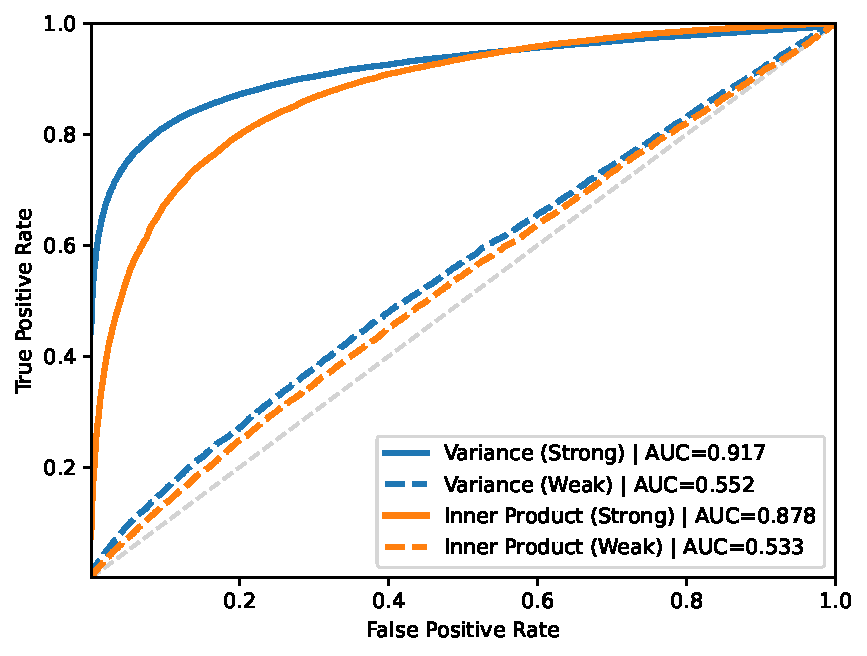
\includegraphics[width=0.7\columnwidth]{figs/celeba_roc_pers.pdf}
%     \caption{ROC of our Task-Inference Attacks on CelebA (Personalization)}
%     \label{fig:celeba}
% \end{figure}


\begin{figure}[t]
    \centering
    \begin{subfigure}[b]{0.32\columnwidth}
        \centering
        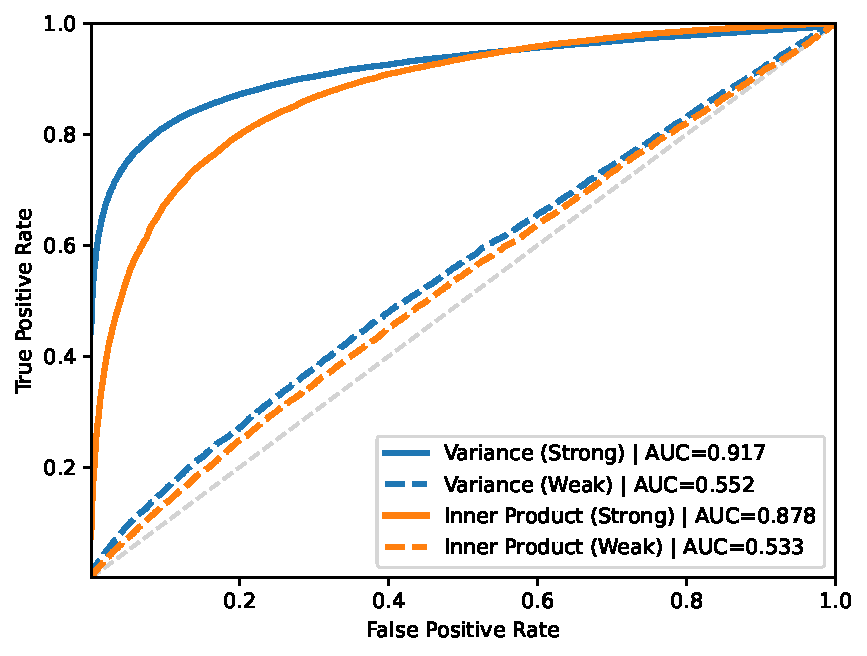
\includegraphics[width=\textwidth]{figs/celeba_roc_pers.pdf}
        \caption{CelebA}
        \label{fig:celeba}
    \end{subfigure}
    % \quad
    \hfill
    \begin{subfigure}[b]{0.32\columnwidth}
        \centering
        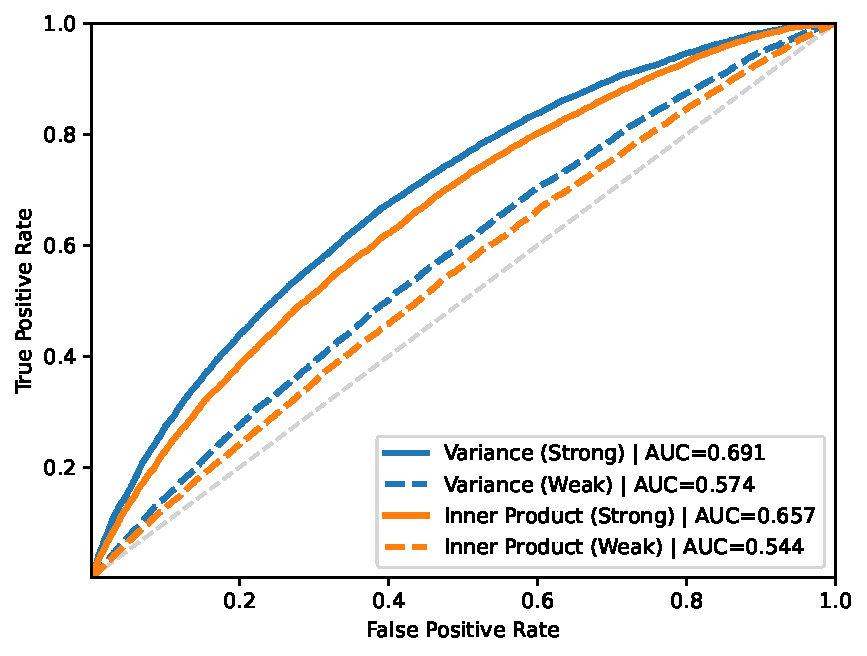
\includegraphics[width=\textwidth]{figs/femnist_roc.pdf}
        \caption{FEMNIST}
        \label{fig:femnist}
    \end{subfigure}
    % \quad
    \hfill
    \begin{subfigure}[b]{0.34\columnwidth}
        \centering
        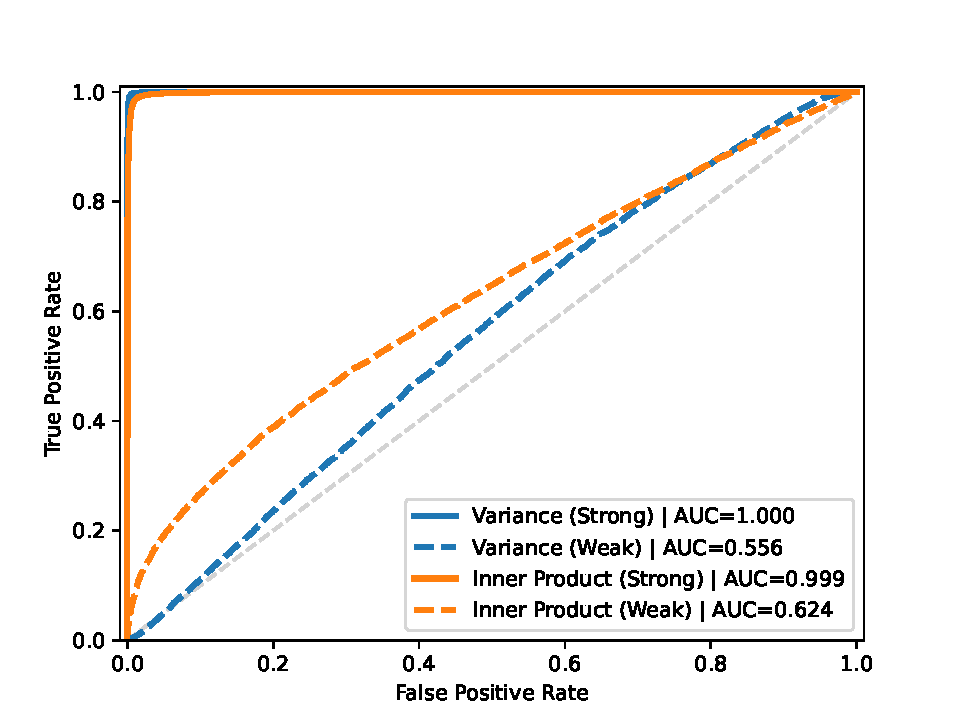
\includegraphics[width=\textwidth]{figs/bertsmall_stackoverflow_128.pdf}
        \caption{Stack Overflow}
        \label{fig:user_level_lm}
    \end{subfigure}
    \caption{ROC of Task-Inference Attacks (Personalization)}
    \label{fig:personalization_roc}
\end{figure}



\subsection{Personalization} \label{sec:personalization}

Here, we present the results of our experiments in the vision and language settings where MTL is used for \textit{personalization}. Across all experiments, the datasets are organized by individual users, with each user contributing multiple samples. In the MTL framework, the multiple tasks are the users, and each user's task-specific layer, which is linear in this case, receives updates from their data. In a distributed learning setting, this could be thought of as locally adapting the model to user-specific data. The shared representation is trained on all of the tasks. When the adversary infers a task's inclusion in multitask training, they are leaking whether or not an individual's data was present at all in updates to the shared representation. Like in membership-inference, the \textbf{strong} adversary will have a batch of real training samples at their disposal to perform this test, but the \textbf{weak} adversary receives fresh samples that belong to the user and were never seen during training.




% \begin{table}
%   \caption{TPR and FPR for Percentile Thresholds for Inner Product Attack~(Personalization)}
%   \label{tab:percentiles_personalization}
%   \begin{tabular}{lcccc}
%     \toprule
%     Dataset&Threshold \%&TPR&FPR&Accuracy\\
%     \midrule
%     CelebA (Fig~\ref{fig:celeba}) & temp& temp&temp&temp\\
%     FMNIST (Fig~\ref{fig:celeba}) & temp& temp&temp&temp\\
%     Stack Overflow (Fig~\ref{fig:user_level_lm}) & temp &temp&temp&temp\\
%   \bottomrule
% \end{tabular}
% \end{table}

\begin{center}
    \begin{table}
    \centering
  \caption{(TPR, FPR) and Balanced Accuracy for Black-Box Percentile Thresholds for Inner Product Attack at $50^{th}$, $75^{th}$, and $90^{th}$ Percentile Thresholds~(Personalization)}
  \label{tab:percentiles_personalization}
  \resizebox{0.9\linewidth}{!}{%
        \begin{tabular}{ll cc cc cc}
            \toprule
            & & \multicolumn{2}{c}{$50^{th}$ Percentile} & \multicolumn{2}{c}{$75^{th}$ Percentile} & \multicolumn{2}{c}{$90^{th}$ Percentile} \\
            Dataset & Access & (TPR, FPR) & Acc. & (TPR, FPR) & Acc. & (TPR, FPR) & Acc. \\
            \midrule
            \multirow{2}{*}{CelebA (Fig~\ref{fig:celeba})} 
            & \textbf{Strong} & $(80\%, 20\%)$ & $80\%$ & $(46.7\%, 3.3\%)$ & $71.7\%$ & $(19.5\%, 0.5\%)$ & $59.5\%$ \\
            & \textbf{Weak} &$(52.4\%, 47.6\%)$ & $52.4\%$ & $(27.4\%, 22.5\%)$ & $52.5\%$ & $(11.5\%, 8.5\%)$ & $51.6\%$ \\
            \midrule
            \multirow{2}{*}{FEMNIST (Fig~\ref{fig:femnist})} 
            & \textbf{Strong} & $(61.1\%, 38.8\%)$ & $61.1\%$ & $(33.5\%, 16.4\%)$ & $58.7\%$ & $(14.3\%, 5.7\%)$ & $54.3\%$\\
            & \textbf{Weak} &$(53.2\%, 46.8\%)$ & $53.2\%$ & $(27.2\%, 22.8\%)$ & $52.2\%,$ & $(11.2\%, 8.8\%)$ & $51.2\%$ \\
            \midrule
            \multirow{2}{*}{Stack Overflow (Fig~\ref{fig:user_level_lm})} 
            & \textbf{Strong} & $(98.7\%, 1.2\%)$ & $98.7\%$ & $(50.0\%, 0\%)$ & $75.0\%$ & $(19.9\%, 0\%)$ & $59.9\%$ \\
            & \textbf{Weak} & $(58.2\%, 41.7\%)$ & $58.2\%$ & $(34.1\%, 15.8\%)$ & $59.1\%$ & $(16.3\%, 3.6\%)$ & $56.3\%$ \\
            \bottomrule
        \end{tabular}
    }
    \end{table}
\end{center}


% celeba 
%strong {'quantile': [0.5, 0.75, 0.9], 'tpr': [80\%, 46.7\%, 19.5\%], 'fpr': [20.0\%3390625, 03.3\%, 0.5\%], 'acc': [80\%, 71.7\%, 59.5\%]}
% weak {'quantile': [0.5, 0.75, 0.9], 'tpr': [52.4\%, 27.4\%74375, 11.5\%2], 'fpr': [47.5\%, 22.5\%, 08.5\%], 'acc': [52.4\%10805253, 52.\%78985605, 51.6\%]}
% @ 1% FPR weak=2% strong=28.2%

% femnist stats (3% TPR @ 1% FPR - strong)
% strong = {'quantile': [0.5, 0.75, 0.9],
%  'tpr': [61.1\%, 33.5\%, 14.3\%],
%  'fpr': [38.8\%, 16.4\%, 5.7\%],
%  'acc': [61.1\%, 58.7\%, 54.3\%]}
% weak = {'quantile': [0.5, 0.75, 0.9],
%  'tpr': [53.2\%, 27.2\%, 11.2\%],
%  'fpr': [46.8\%, 22.8\%, 08.8\%],
%  'acc': [53.2\%, 52.2\%, 51.2\%]}




% stackoverflow stats to add

% strong = {'quantile': [0.5, 0.75, 0.9],
%  'tpr': [98.7\%, 50.0\%, 19.9\%],
%  'fpr': [01.2\%, 0,. \%0].,\%
%  'acc': [98.7\%, 75.0\%, 59.9\%]}
% weak = {'quantile': [0.5, 0.75, 0.9],
%  'tpr': [58.2\%, 34.1\%, 16.3\%],
%  'fpr': [41.7\%, 15.8\%, 03.6\%],
%  'acc': [58.2\%, 59.1\%, 56.3\%]}



\subsubsection{CelebA} \label{sec:celeba}

First, we report the results for our attacks in the vision setting. We train a ResNet34~\cite{ResNet} from an ImageNet~\cite{imagenet} checkpoint with one linear layer per task on the CelebA~\cite{liu-2015-celeba} dataset to perform binary facial attribute detection, with each task corresponding to a person in the dataset. We filter CelebA such that each unique individual has roughly 30 images containing their face, and we hold out 8 samples per individual to mount an attack with the \textbf{weak} adversary. In our experiments, we jointly train the MTL model on 256 total tasks with 22 samples per task, or roughly 5600 total samples, and thus use several regularization techniques to ensure that the ResNet layers learn performant embeddings. During each training step, we randomly sample a batch of tasks and update their corresponding task heads, while aggregating these tasks' gradients to update the shared representation.

Once the model is trained, we run 128 trials of each attack on all 512 tasks (256 $IN$ and 256 $OUT$), using 8 samples per task for the \textbf{strong} adversary and 4 of the held out samples per task for the \textbf{weak} adversary. The results of this experiment are shown in Figure~\ref{fig:celeba} and Table~\ref{tab:percentiles_personalization}. We find that while both the \textbf{strong} and \textbf{weak} adversaries can achieve non-trivial success rates in determining a task's inclusion in training, the true positive rate of the \textbf{weak} adversary is bounded above by the true positive rate of the \textbf{strong} adversary for any fixed FPR. Moreover, we see that our variance attack nets better TPR in the low FPR regime, but the inner product attack sees better FPR at higher FPR. At a fixed FPR of $1\%$, the TPR of our variance attack on CelebA achieves a TPR of $61.2\%$  and  $2.9\%$ for the for the \textbf{strong} and \textbf{weak} adversaries, respectively.


\subsubsection{FEMNIST} \label{sec:femnist}

We report additional results in the vision setting for Federated EMNIST~\cite{caldas-2019-leafbenchmark}. We train a MTL model with ResNet8~\cite{ResNet} as the shared representation and personalize each task-specific layer to a unique writer in the dataset. Each writer in the FEMNIST has much more data than each individual in CelebA. Thus, we train the MTL model on 128 tasks with 128 samples per task and hold out 16 samples to mount our attack with the \textbf{weak} adversary. For each of the 128 runs of the attack, the \textbf{strong} adversary receives 16 training samples, and the \textbf{weak} adversary receives 8 of the held out samples. Figure~\ref{fig:femnist} and Table~\ref{tab:percentiles_personalization} show the ROC curves and (TPR, FPR) pairs of our task-inference attacks on Federated EMNIST. We observe that both the \textbf{strong} and \textbf{weak} adversaries are able to achieve nontrivial success rates, and the \textbf{strong} adversary sees a TPR of 3\% at a fixed 1\% FPR. When the \textbf{weak} adversary picks the $90^{th}$ percentile threshold, the inner product attack yields a 2.5$\times$ higher TPR than FPR.


% \begin{figure}[h]
%     \centering
%     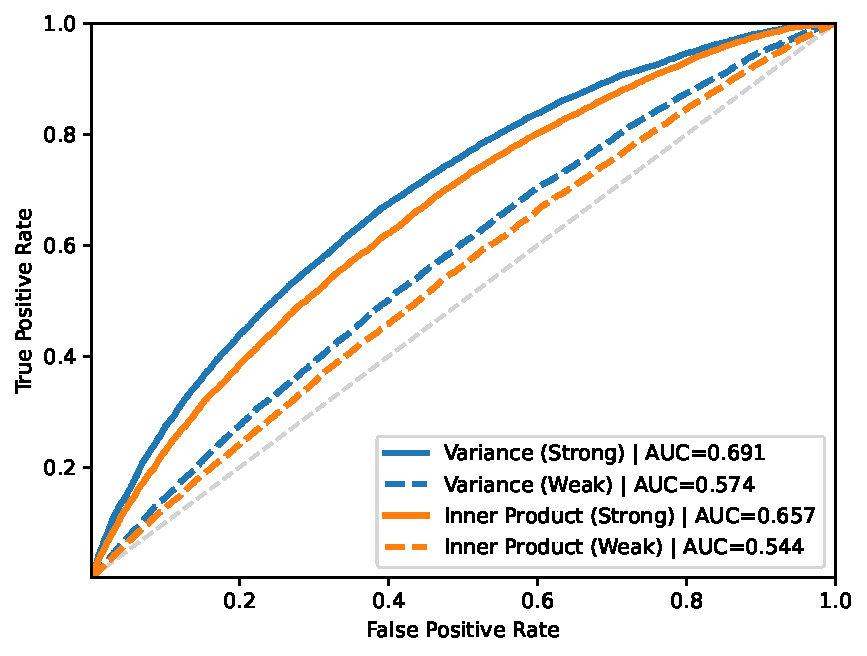
\includegraphics[width=0.5\columnwidth]{figs/femnist_roc.pdf}
%     \caption{ROC of our Task-Inference Attacks on FEMNIST (Personalization)}
%     \label{fig:femnist}
% \end{figure}




\subsubsection{Stack Overflow} \label{sec:stackoverflow}


Next, we present the results for our language experiments on the StackOverflow posts dataset. We train a BERT Small~\cite{bertsmall_1} (29M parameters) to perform topic classification, where the tasks are users who contributed posts to Stack Overflow. We filter the dataset such that each individual has at least 48 total posts; 32 posts for the model's training set and 16 to be used by the \textbf{weak} adversary. Then, we split the dataset into 128 \textbf{IN} tasks and 128 \textbf{OUT} tasks, yielding two datasets of roughly 10k posts, with each user contributing about 140 posts on average. We train the shared representation and task-specific linear layers jointly on the \textbf{IN} dataset. The MTL model is trained to detect the presence of 256 unique topics in posts, and each post can have multiple corresponding topics. 

After training is complete, we run each attack on all 256 tasks for 128 trials, using 8 samples and 4 samples per trial for the \textbf{strong} and \textbf{weak} adversary, respectively. Figure~\ref{sec:stackoverflow} and Table~\ref{tab:percentiles_personalization} show the results for this attack. We find that the \textbf{strong} adversary achieves nearly perfect AUC for both attacks and FPR of 0\% at the $75^{th}$ and $90^{th}$ percentile thresholds over all runs of the attack. The \textbf{weak} adversary again sees nontrivial AUC for both attacks, and we see a tradeoff between the TPR of the variance and inner product attacks at particularly high FPR. At fixed FPR of 1\% the inner product adversary with \textbf{weak} access to the data achieves a TPR of 8.2\%, while the \textbf{strong} adversary achieves a TPR of 98.5\%. By analyzing the topic frequencies in the dataset, we empirically find that individual users tend to only write about a small subset of topics. Across all posts, the median user posts about 31 (or 12.1\%) of the 256 total topics, which could lead to high distinguishability of users in representation space.


% \begin{figure}[h]
%     \centering
%     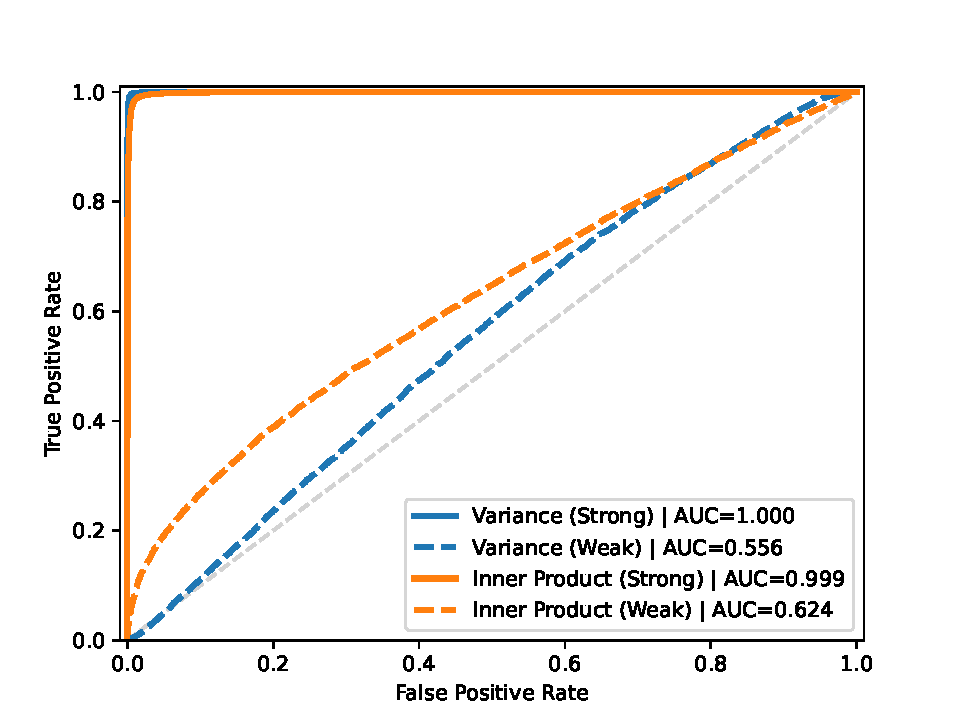
\includegraphics[width=0.7\columnwidth]{figs/bertsmall_stackoverflow_128.pdf}
%     \caption{ROC of Task-Inference Attacks on Stack Overflow (Personalization)}
%     \label{fig:user_level_lm}
% \end{figure}

\subsubsection{Variance Attack Test Statistic} Across all of our experiments in both MTL settings, the statistic produced by our inner product attack (Algorithm~\ref{alg:inner_attack}) is consistent with respect to the ordering of \textbf{IN} and \textbf{OUT} distributions. In contrast, when studying leakage in MTL for personalization, we observe a discrepancy in the test statistic distributions for vision and language datasets. Figure~\ref{fig:hist_difference} shows that the coordinate-wise variance statistic (Algorithm~\ref{alg:var_attack}) is larger for \textbf{IN} tasks than \textbf{OUT} tasks. In Appendix~\ref{appdx:variance_attack}, we find that MTL training of ResNet models produces task heads which are positively correlated, while our BERT models produce nearly orthogonal task-specific layers. Because the task heads are correlated, the primary signal for our attack is the shared representation's "overconfidence" in certain directions of the embedding space, which yields higher coordinate-wise variance. We find that the task heads of our FEMNIST models have the highest correlation, followed by our CelebA models, then Stack Overflow, which maps to the ordering of the AUC scores we see in our experiments on MTL for personalization.

\begin{figure}[h]
    \centering
    \begin{subfigure}[h]{0.35\columnwidth}
        \centering
        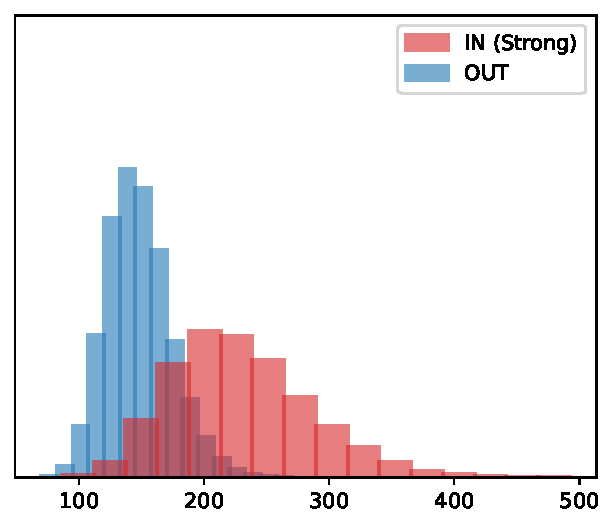
\includegraphics[width=\textwidth]{figs/celeba_hist.pdf}
        \caption{CelebA}
        \label{fig:celeba_hist}
    \end{subfigure}
    \quad \quad
    \begin{subfigure}[h]{0.35\columnwidth}
        \centering
        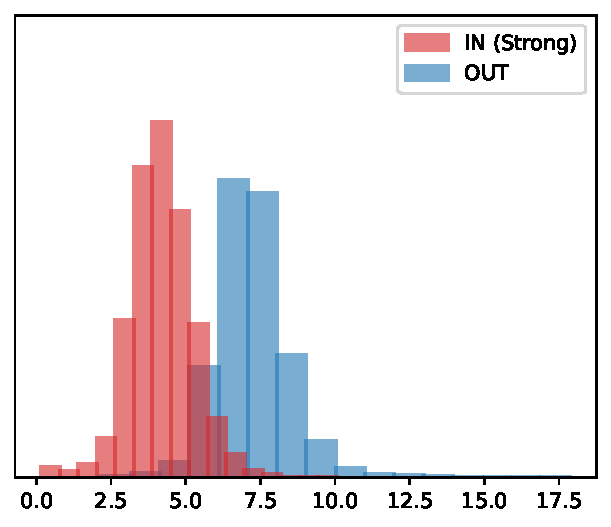
\includegraphics[width=\textwidth]{figs/multilbl_stackoverflow_hist.pdf}
        \caption{Stack Overflow}
        \label{fig:so_hist}
    \end{subfigure}
    \caption{Distribution of Coordinate-Wise Variance Statistic}
    \label{fig:hist_difference}
\end{figure}

% \begin{table*}[t]
%     \centering
%     \caption{TPR and FPR for Black-Box Percentile Thresholds for Inner Product Attack at $(50^{th}$, $75^{th}$, and $90^{th})$ Percentile Thresholds~(Multiple Learning Problems)}
%     \label{tab:percentiles_task_level}
%     \begin{tabular}{llccc}
%         \toprule
%         Dataset & Access & TPRs & FPRs & Accuracies \\
%         \midrule
%         \multirow{2}{*}{CelebA (Fig~\ref{fig:task_level_celeba})} 
%           & \textbf{Strong} & &  & \\
%           & \textbf{Weak}   &   &  & \\
%         \midrule
%         \multirow{2}{*}{Stack Overflow (Fig~\ref{fig:task_level_lm})} 
%           & \textbf{Strong} & $(87\%, \: 48.3\%, \: 19.9\%)$ & $(13.9\%, \: 1.7\%, \:, 0.1\%)$ & $(87\%, \: 73.3\%, \: 59.9\%)$ \\
%           & \textbf{Weak}   & $(85.9\%, \: 47.6\%, \: 19.6\%)$  & $(14.1\%, \: 2.4\%, \:, 0.2\%)$ & $(85.9\%, \: 72.6\%, \: 59.7\%)$ \\
%         \bottomrule
%     \end{tabular}
% \end{table*}

\begin{table*}[t]
    \centering
    \caption{(TPR, FPR) and Balanced Accuracy for Black-Box Percentile Thresholds for Inner Product Attack at $50^{th}$, $75^{th}$, and $90^{th}$ Percentile Thresholds~(Multiple Learning Problems)}
    \label{tab:percentiles_task_level}
    \resizebox{0.88\linewidth}{!}{
        \begin{tabular}{ll cc cc cc}
            \toprule
            & & \multicolumn{2}{c}{$50^{th}$ Percentile} & \multicolumn{2}{c}{$75^{th}$ Percentile} & \multicolumn{2}{c}{$90^{th}$ Percentile} \\
            Dataset & Access & (TPR, FPR) & Acc. & (TPR, FPR) & Acc. & (TPR, FPR) & Acc. \\
            \midrule
            \multirow{2}{*}{CelebA (Fig~\ref{fig:task_level_celeba})} 
              & \textbf{Strong} & $(68.9\%, 31.1\%)$  & $68.9\%$ & $(42.6\%, 7.4\%)$ & $67.6\%$ & $(22.8\%, 0\%)$ & $61.4\%$ \\
              & \textbf{Weak}   & $(52.5\%, 47.5\%)$ & $52.5\%$ & $(29.0\%, 21.0\%)$ &  $54\%$ & $(13.5\%, 6.6\%)$  & $53.5\%$ \\
            \midrule
            \multirow{2}{*}{Stack Overflow (Fig~\ref{fig:task_level_lm})} 
              & \textbf{Strong} & $(87\%, 13.9\%)$ & $87\%$ & $(48.3\%, 1.7\%)$ & $73.3\%$ & $(19.9\%, 0.1\%)$ & $59.9\%$ \\
              & \textbf{Weak}   & $(85.9\%, 14.1\%)$ & $85.9\%$ & $(47.6\%, 2.4\%)$ & $72.6\%$ & $(19.6\%, 0.2\%)$ & $59.7\%$ \\
            \bottomrule
        \end{tabular}
    }
\end{table*}


% celeba = 
% Strong 0.5th Percentile: TPR=68.9\%, FPR=31.1\%, ACC=68.9\%
% Strong 0.75th Percentile: TPR=42.6\%, FPR=07.4\%, ACC=67.6\%
% Strong 0.9th Percentile: TPR=22.8\%, FPR=0\%, ACC=61.42\%

% Strong 0.5th Percentile: TPR=52.5\%, FPR=47.5\%, ACC=52.5\%
% Strong 0.75th Percentile: TPR=29.0\%, FPR=21.0\%, ACC=54.0\%
% Strong 0.9th Percentile: TPR=13.5\%, FPR=06.6\%, ACC=53.5\%

\subsection{Multiple Learning Problems} \label{sec:multiple_obj}

We present the results of our experiments on models trained using MTL on multiple related learning problems. In contrast to the datasets used to train MTL models in the experiments presented from Section~\ref{sec:personalization}, the datasets are split by learnable classes in the dataset rather than by person. For example, Stack Overflow can be split into its constituent topics, and we can have an MTL model with a tailored head for detecting each individual topic's presence. We draw attention to the fact that in this setting, the labels for the learning problem are directly tied to the task. In other words, if a task is not included, there are no positive labels corresponding to that task in the training dataset. In our experiments on personalized multitask models, while there is some dependency between the task and the labeling of the data (e.g. a celebrity in CelebA with blonde hair is classified as "Blonde" 100\% of the time), there is not a direct mapping from the data's labeling to the tasks in MTL. 


\subsubsection{CelebA} \label{sec:celeba_task_level}

For our evaluation on CelebA, we split the dataset into potentially overlapping tasks by facial attribute, 20 \textbf{IN} and 20 \textbf{OUT}, with at least 1024 samples with corresponding positive and negative labelings for each task. Because some tasks have very low positive label frequencies (e.g. < 1\%), this minimum sample size ensures sufficient positive examples for the task head to learn from. We use the ResNet50~\cite{ResNet} architecture as the backbone for our MTL model as there is ample data. Each task has a corresponding linear head for binary attribute prediction, and no two tasks share the same labeling. For example, the task head dedicated to hair color does not make predictions for the task head dedicated to detecting glasses. 

We average the results of our experiments over 8 MTL runs, and run the attacks on the 40 total tasks 128 times each, using 16 samples and 8 samples for the \textbf{strong} and \textbf{weak} adversary, respectively. In Table~\ref{tab:percentiles_task_level} and Figure~\ref{fig:task_level_celeba}, we see that the \textbf{strong} adversary is able to achieve an AUC of $0.745$ using our coordinate-wise variance attack and a TPR of 22.8\% at an empirical FPR of 0\% over all runs when using the $90^{th}$ percentile threshold. The \textbf{weak} sees nontrivial success rates, with a TPR roughly 2$\times$ larger than the FPR when using the $90^{th}$ percentile threshold. 





\subsubsection{Stack Overflow} \label{sec:stack_overflow_task_level}


We also run our attack on language models where MTL is used for multiple related learning problems. Unlike the experiments in Section~\ref{sec:stackoverflow}, the posts are not split by user. Instead, each task corresponds to the inclusion of a positively labeled topic in the dataset. For example, if the Stack Overflow topic "Python" is \textbf{IN}, there is a task head dedicated to detecting whether a post includes the topic "Python". If the topic is \emph{not} included, there is no task head that can learn positively labeled "Python" samples. Additionally, because the posts in the Stack Overflow dataset can contain multiple topics, the training data is not disjoint between tasks; the labeling of each task dataset is unique. We randomly split the data into 70 \textbf{IN} tasks and 70 \textbf{OUT} tasks, with each task-specific dataset containing 1024 posts. Using a BERT Medium~\cite{bertsmall_1} (41M parameters) model as the shared representation, we use MTL to learn linear task heads that are specialized to detecting the presence of a single topic within a post.

We run both of our attacks on the BERT model 128 times, using 32 samples and 16 samples each trial for the \textbf{strong} and \textbf{weak} adversaries, respectively. Figure~\ref{fig:task_level_lm} shows that in the setting where tasks correspond directly to the training data labeling in MTL, the gap in attack performance between the \textbf{strong} and \textbf{weak} adversaries becomes small. This can be attributed to the fact that the model necessarily has to achieve high utility on the training tasks in order to solve the learning problems. This contrasts our findings in Section~\ref{sec:personalization}, where the task heads in MTL are not solving distinct learning problems, and the separation between both adversaries is notably larger. In Table~\ref{tab:percentiles_task_level}, we see that the (TPR, FPR) pairs for both adversaries are nearly equal, and the \textbf{weak} adversary is able to achieve a 19.6\% TPR at 0.2\% FPR. 

% \begin{figure}[h]
%     \centering
%     \begin{subfigure}[h]{0.35\columnwidth}
%         \centering
%         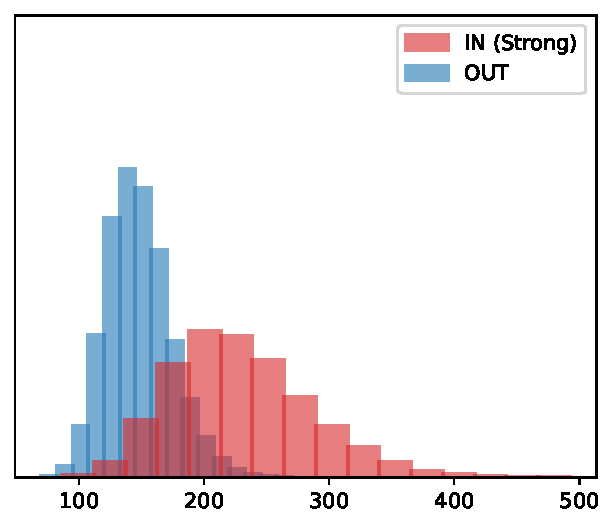
\includegraphics[width=\textwidth]{figs/celeba_hist.pdf}
%         \caption{CelebA}
%         \label{fig:celeba_hist}
%     \end{subfigure}
%     \quad \quad
%     \begin{subfigure}[h]{0.35\columnwidth}
%         \centering
%         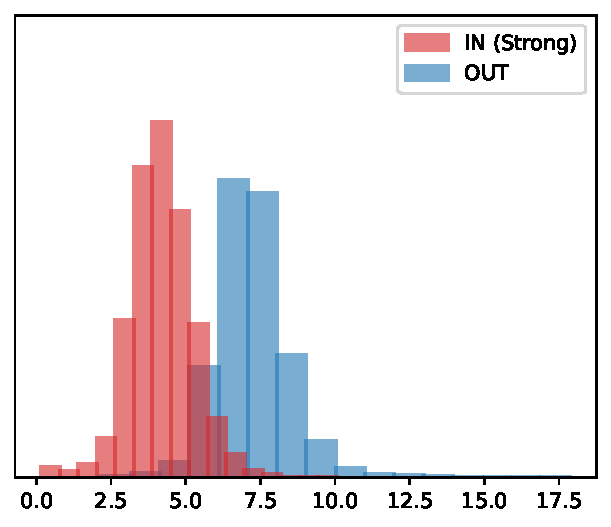
\includegraphics[width=\textwidth]{figs/multilbl_stackoverflow_hist.pdf}
%         \caption{Stack Overflow}
%         \label{fig:so_hist}
%     \end{subfigure}
%     \caption{Distribution of Coordinate-Wise Variance Statistic}
%     \label{fig:hist_difference}
% \end{figure}

\begin{figure}[ht]
    \centering
    \begin{subfigure}[b]{0.44\textwidth}
        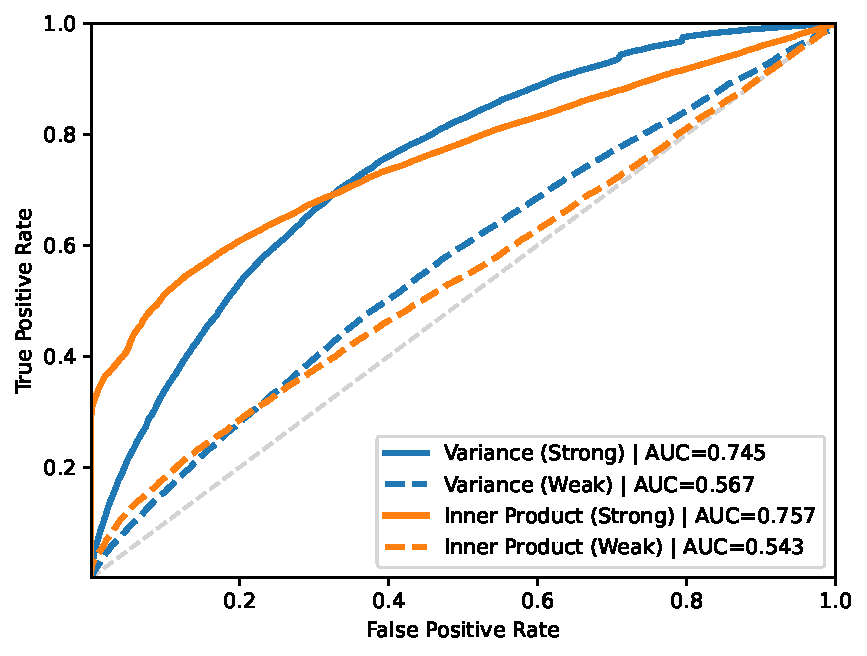
\includegraphics[width=\textwidth]{figs/task_lvl_celeba.pdf}
        \caption{CelebA}
        \label{fig:task_level_celeba}
    \end{subfigure}
    \hfill
    \begin{subfigure}[b]{0.44\textwidth}
        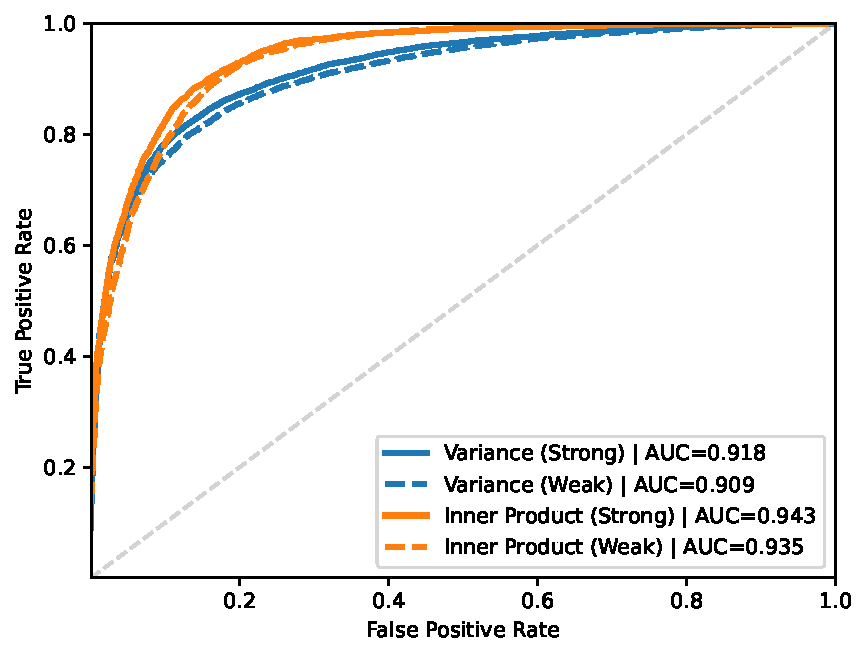
\includegraphics[width=\textwidth]{figs/task_level_inference_language.pdf}
        \caption{Stack Overflow}
        \label{fig:task_level_lm}
    \end{subfigure}    
    \caption{ROC of Task-Inference Attacks (Multiple Learning Problems)}
    \label{fig:task_inference}
\end{figure}
    

\subsection{Investigating Sources of Task-Inference Leakage}  Now, we present an investigation of the factors that lead to task-inference. We study how task-inference success varies as a function of gaps between the MTL model's loss on training samples, out of sample data, and out of distribution data. In Appendix~\ref{appdx:synth}, we conduct ablation studies over MTL parameters, such as the embedding dimension and number of tasks, using a synthetic dataset designed to necessitate MTL.

\subsubsection{Task-Inference and Generalization}




The \textbf{weak} adversary in our analysis of tracing attacks for task-inference (Theorem~\ref{thm:weak_adv}) has a notable disadvantage compared to the \textbf{strong adversary}, which has access to actual training samples. When estimating a mean of Gaussian vectors, having several tasks with sparse data yields an accurate enough estimate of the true mean such that the gap between the strong and weak adversaries is observable, but not too large. In our MTL experiments, we see that this gap in AUC between the \textbf{strong} and \textbf{weak} adversaries is larger, especially when each individual task has very few samples, such as in CelebA. In membership-inference, the adversary's success rate is often tied to the model's generalization gap~\cite{2018-yeom-mioverfitting} (and in very overparameterized models, the train loss as it approaches 0) as the model's outputs begin to heavily depend on training examples. To understand the relationship between generalization error and task-inference success, we train Stack Overflow topic classification models, using MTL for personalization over 128 users as in Section~\ref{sec:personalization}, and measure the AUC each adversary achieves using the inner product attack. In total, we train 8 MTL models on random splits of 128 tasks and run the attack 128 times per task, using 8 and 4 samples per run for the \textbf{strong} and \textbf{weak} adversaries, respectively.

Figure~\ref{fig:gengap_pers} shows the \textbf{strong} adversary's AUC as a function of the gap between the training loss and "zero-shot" loss, which we compute by taking the average prediction of 16 random task heads to make predictions on \textbf{OUT} task data. Each point on the scatterplot is shaded corresponding to how many epochs the model had been trained up to that point. We observe a similar trend to membership-inference, where our \textbf{strong} task-inference adversary, which has access to training samples, sees a sharp increase in attack AUC for small generalization gaps. Over many runs of model training on different task splits, we see that the points on the plot tend to concentrate as the generalization gap grows.


\begin{figure*}[t]
    \centering
    \begin{subfigure}[b]{0.57\linewidth}
        \centering
        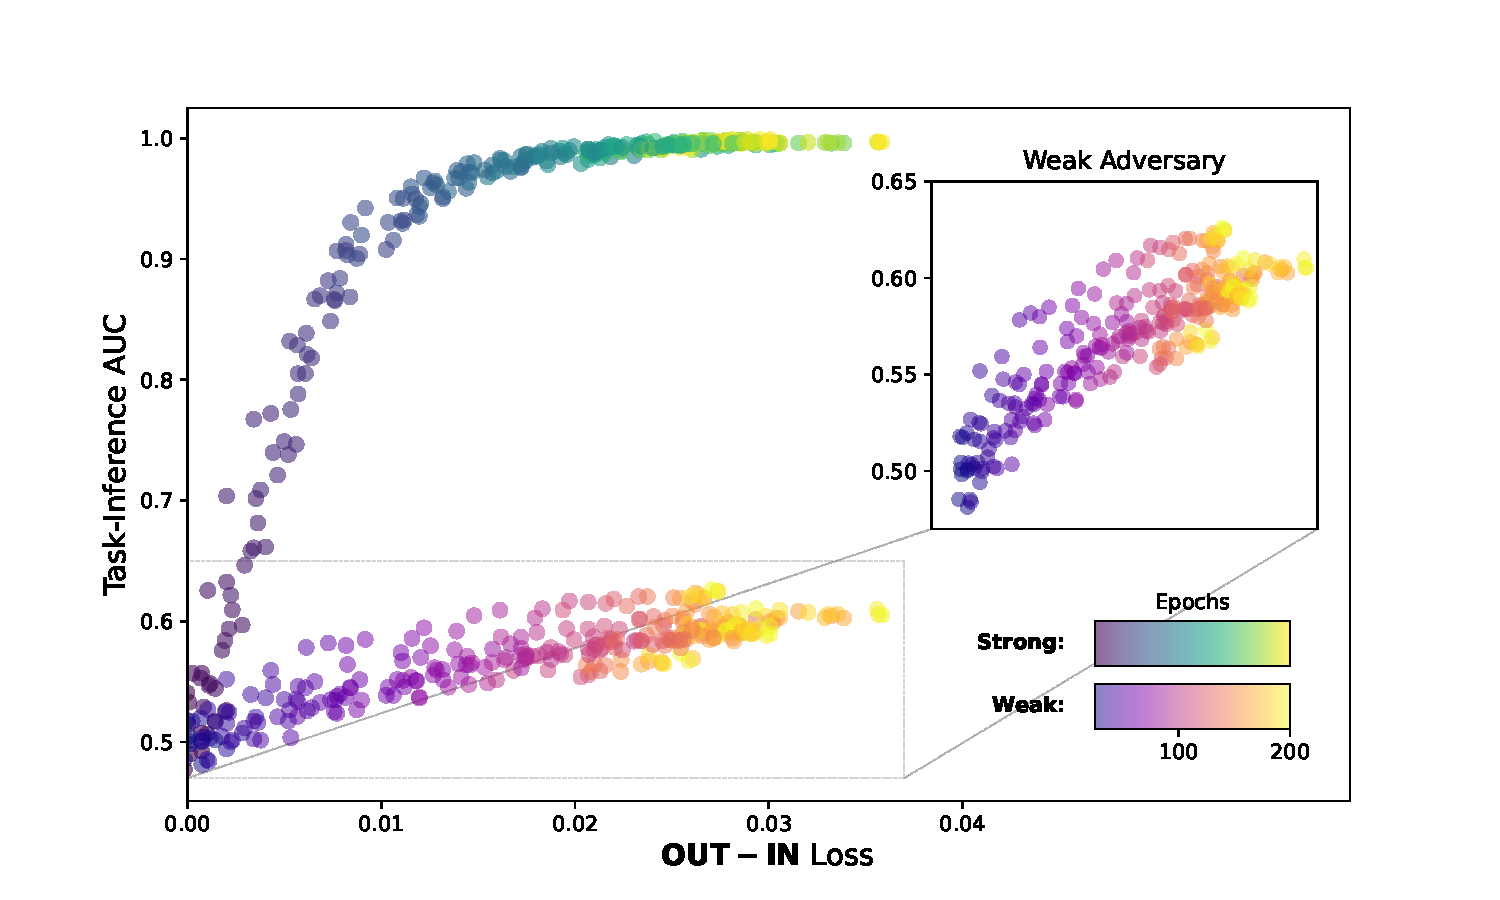
\includegraphics[width=\textwidth]{figs/ablations/gengaps_zoom.pdf}
        \caption{\textbf{Strong} and \textbf{Weak} (Personalization)}
        \label{fig:gengap_pers}
    \end{subfigure}
    % \hfill
    % \begin{subfigure}[b]{0.3\linewidth}
    %     \centering
    %     \includegraphics[width=\textwidth]{figs/ablations/gengaps_weak_pers.pdf}
    %     \caption{Weak (Personalization)}
    %     \label{fig:weak_gengap}
    % \end{subfigure}
    \hfill
    \begin{subfigure}[b]{0.39\linewidth}
        \centering
        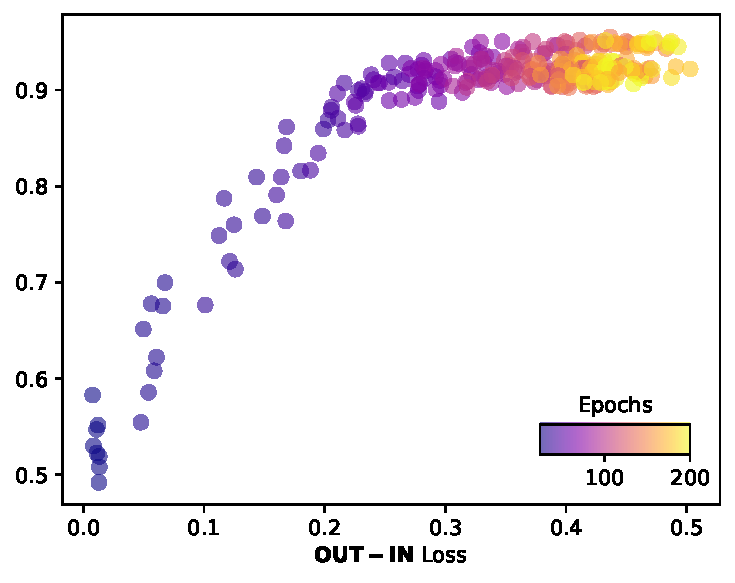
\includegraphics[width=\textwidth]{figs/ablations/gengaps_weak_task_lvl.pdf}
        \caption{\textbf{Weak} (Multiple Learning Problems)}
        \label{fig:weak_gengap_task_level}
    \end{subfigure}
    \caption{Relationship Between Generalization Gaps and Inner Product Attack AUC on Stack Overflow}
    \label{fig:gengaps}
\end{figure*}

In contrast, when we run the exact same experiment with the \textbf{weak} adversary, we see that the attack AUC also grows as a function of the loss gap, but there is more variance. Here, the x-axis is the gap between the "zero-shot" loss and the loss on samples which did \emph{not} appear in training, but belong to training tasks. This observation implies that the model is both generalizing more effectively to tasks, or data distributions, that were seen in training and memorizing some amount of information about the task as a whole, rather than only particular training samples. A similar observation was made for user-inference attacks on generative LLMs in~\cite{kandpal2023userinference}, where the authors observe increasing attack AUC on user as a function of the model's validation loss on \textbf{IN} users. We supplement these findings by running another experiment, shown in Figure~\ref{fig:weak_gengap_task_level}, where the MTL model is trained to solve multiple learning problems at once. In this setting, the labeling of the training data for any task head directly corresponds to the task itself (e.g. the task-specific layer for "Python" only has positively labeled training samples that correspond to posts with the topic "Python"). Our observations highlight that the interdependence between the definition of tasks in an instance of MTL and the learning problems being solved by the task-specific layers has a measurable impact on task-inference AUC as the model becomes well-generalized on tasks included in training.





